% !Mode:: "TeX:UTF-8:Main"

\documentclass{article}
\usepackage{l3pdf}
\usepackage{pdfresources}
\ExplSyntaxOn
\pdf_uncompress:
\ExplSyntaxOff

\usepackage{ifluatex,graphicx}
\usepackage{pdfpages,xcolor}
\usepackage[customdriver=hgeneric-experimental]{hyperref}
\hypersetup{linkbordercolor=red}
\hypupdateattribute

\ifluatex
\directlua{
 require("newpax")
 newpax.writenewpax("pax-input")
 %newpax.writepax("pax-input")
 %newpax.writenewpax("figure/pax-input2")
% newpax.writenewpax("example-image-a")
 %newpax.writenewpax("C:/texlive/2020/texmf-dist/doc/latex/biblatex/biblatex")
 %newpax.writenewpax("C:/texlive/2020/texmf-dist/doc/latex/pgfplots/pgfplots")
 %newpax.writenewpax("C:/texlive/2020/texmf-dist/doc/latex/tools/longtable")
 newpax.writenewpax("tests/pdf_reference_1-7")
 }
\fi

\usepackage{newpax}
%\makeatletter
%\patchcmd\PAX@pdf@annot{\PAX@pagellx}{\PAX@page@llx}{}{\fail}
%\makeatother
\newpaxsetup{paxextension=newpax}

\errorcontextlines200
\begin{document}\raggedright
%\includepdf[pages=-]{C:/texlive/2020/texmf-dist/doc/latex/tools/longtable}
%\includepdf[pages=-]{C:/texlive/2020/texmf-dist/doc/latex/pgfplots/pgfplots}
%\includepdf[pages=-]{tests/pdf_reference_1-7}

included graphic:
%\tracingifs=1 \tracingmacros=1
%\fbox{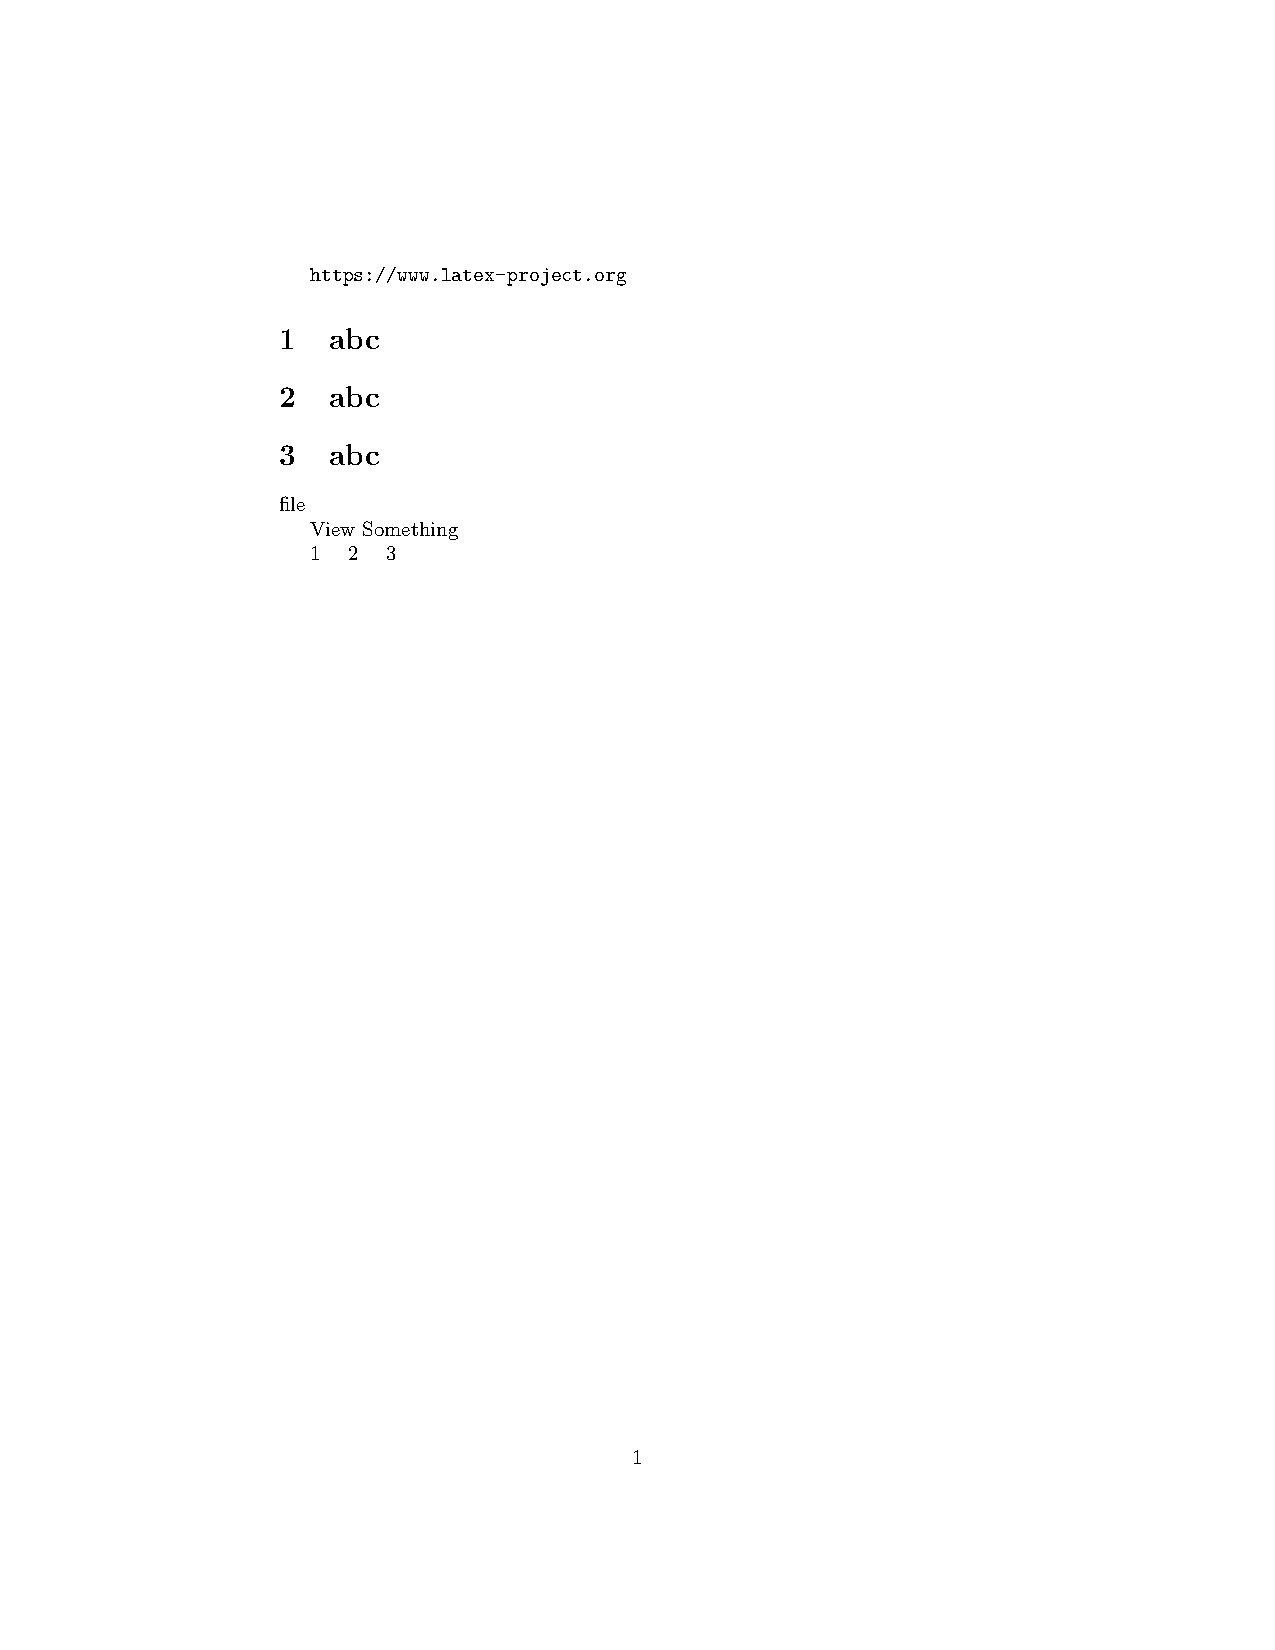
\includegraphics[scale=0.5,trim=4cm 15cm 8cm 3cm,clip,page=1]{pax-input}}
%\fbox{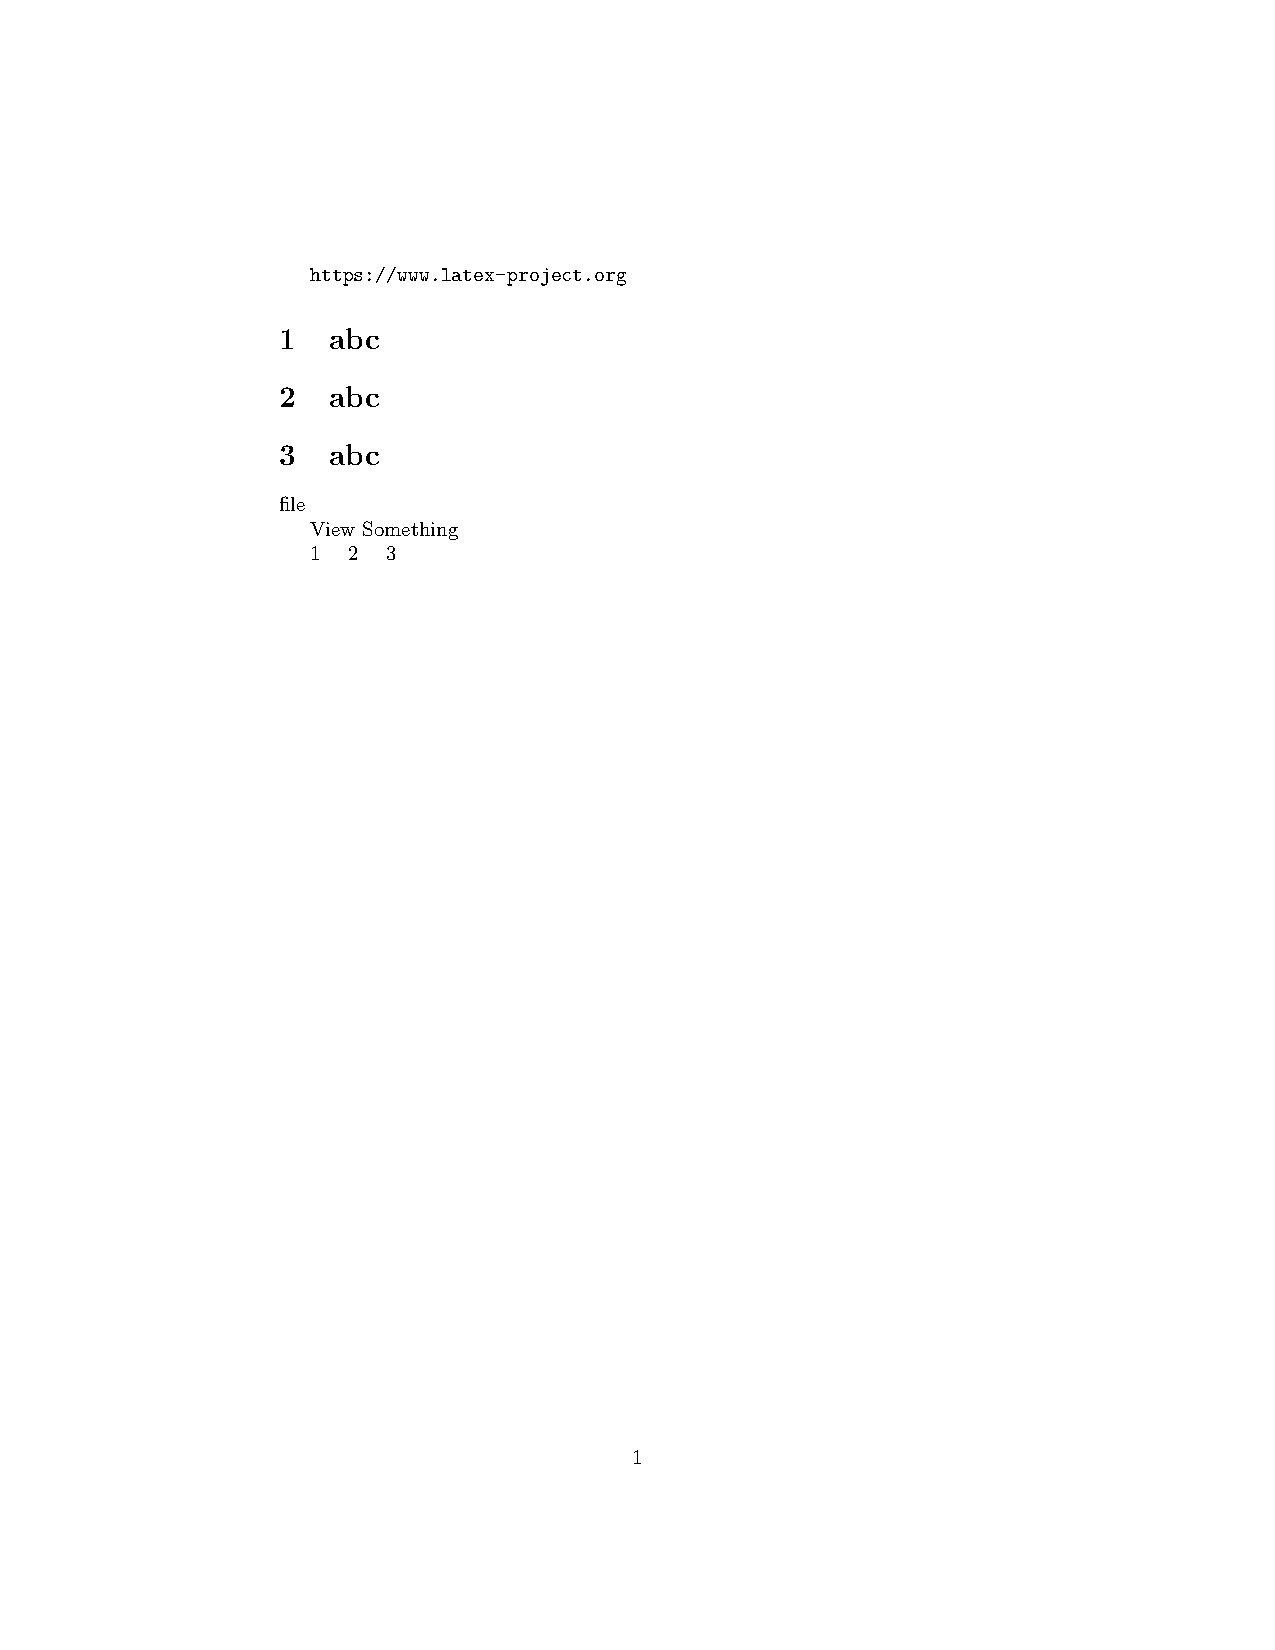
\includegraphics[trim=4cm 15cm 8cm 3cm,clip]{pax-input}}
%\fbox{\includegraphics[page=2]{pax-input}}

%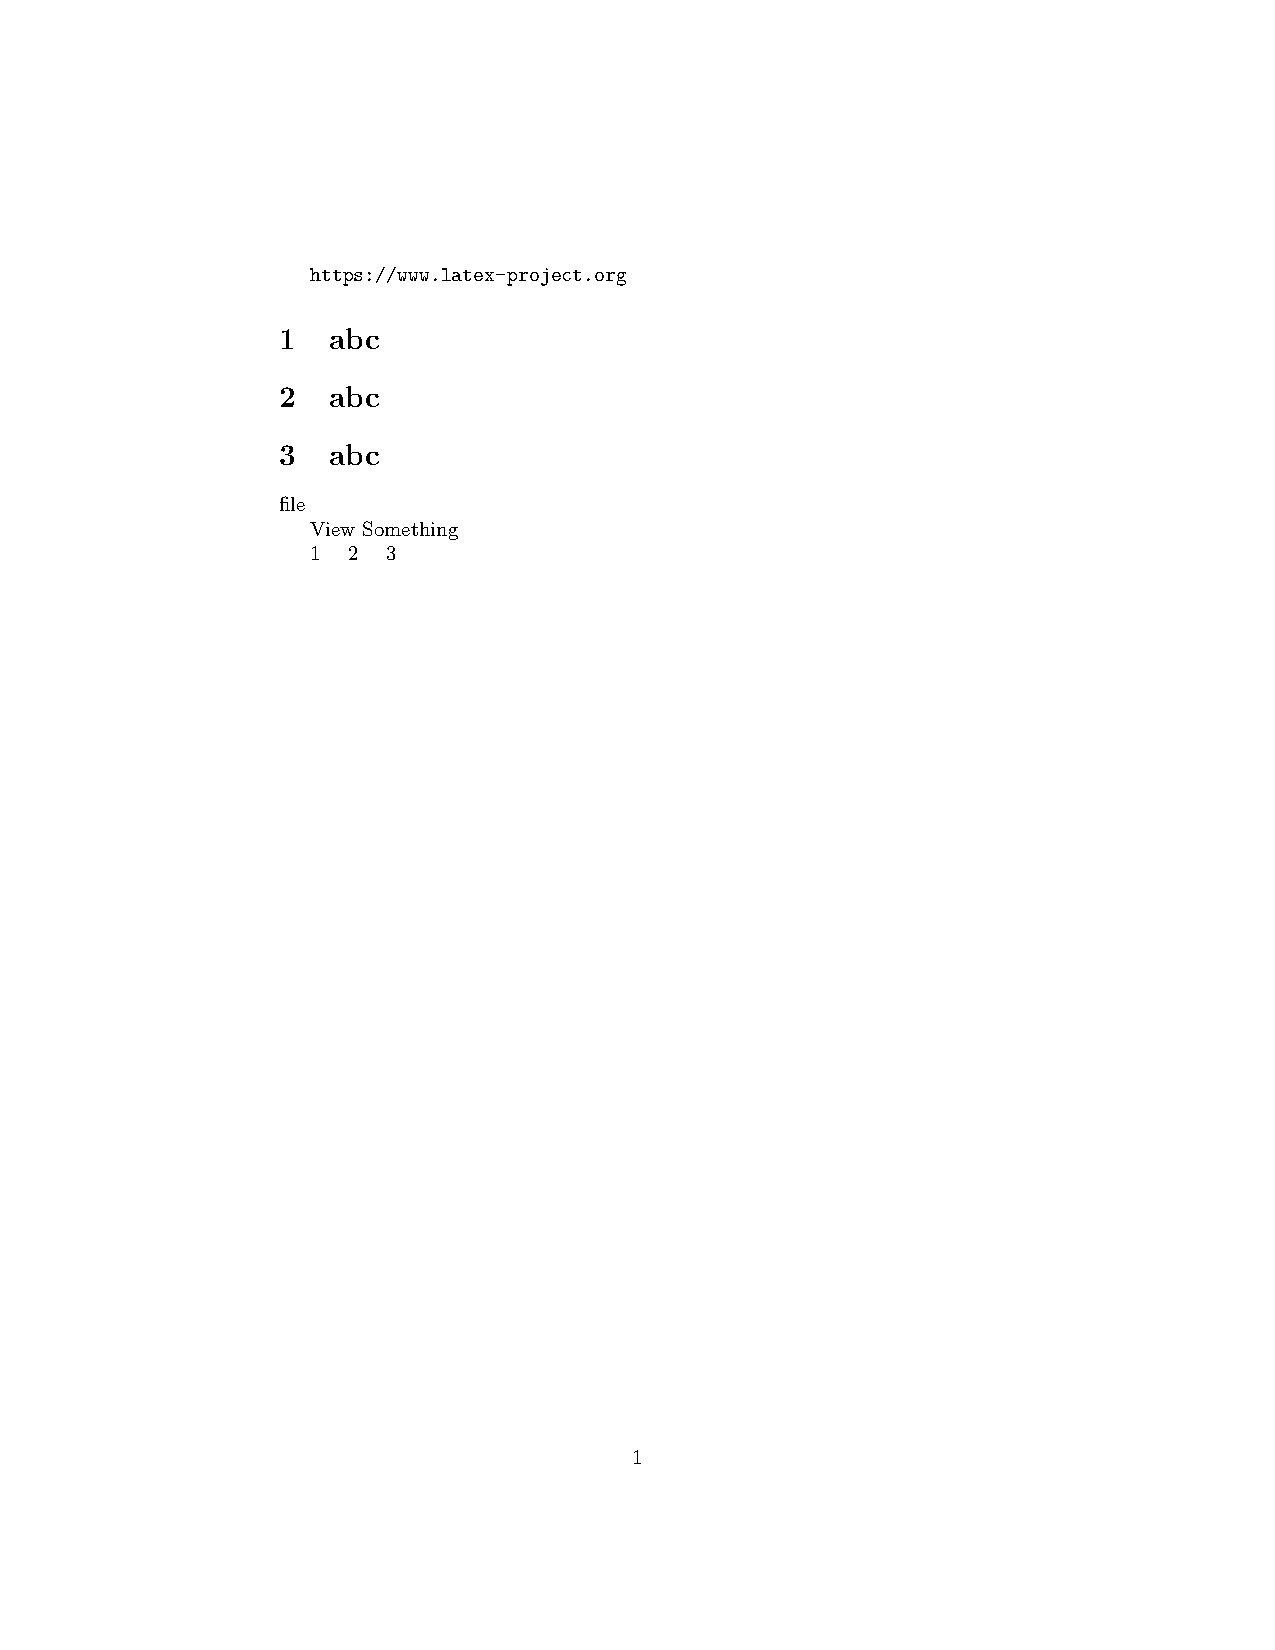
\includepdf{pax-input}
\end{document}
\fbox{\includegraphics[scale=0.5,trim=5cm 15cm 8cm 3cm,clip,page=2]{pax-input}}

%\newpaxsetup{useattributes=false,destsuffix=B}

%\newpaxsetup{addannots=false}
\fbox{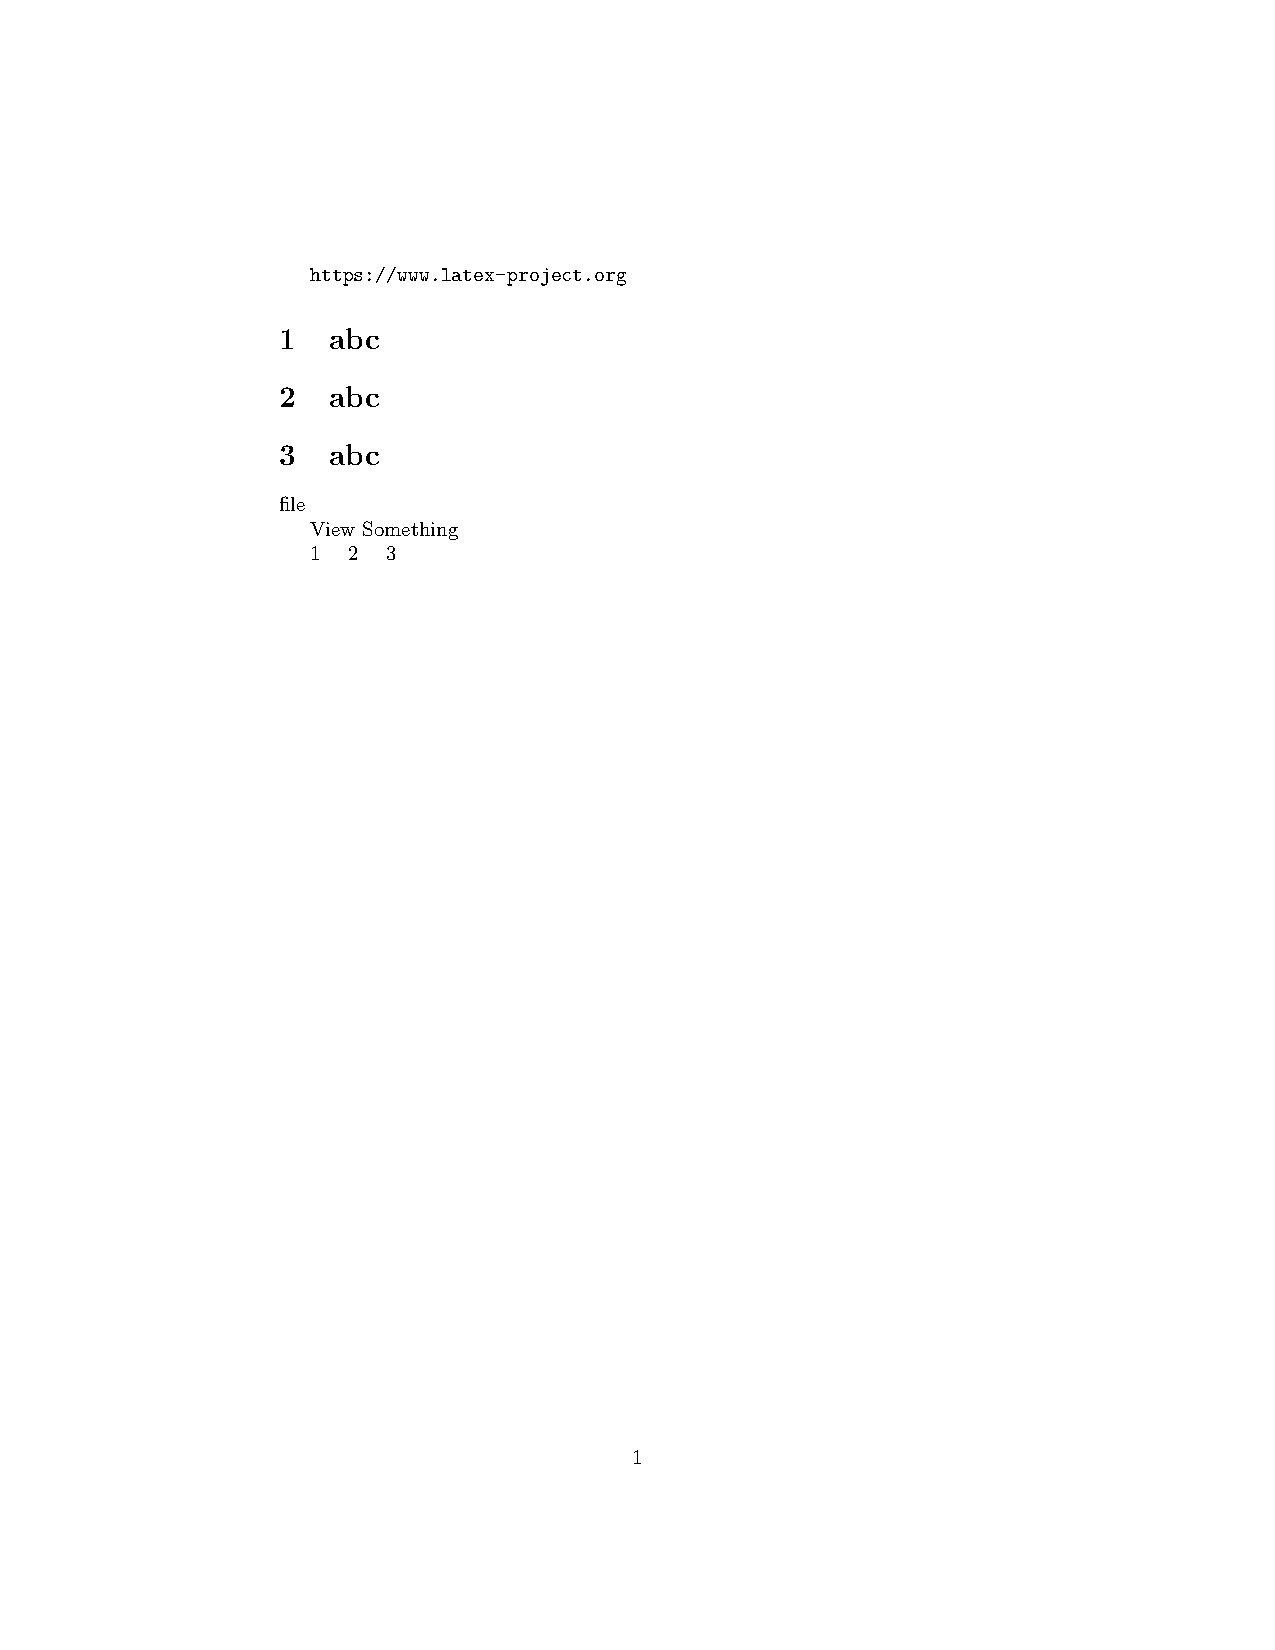
\includegraphics[scale=0.5,trim=4cm 15cm 8cm 3cm,clip,page=1]{pax-input}}

%\newpaxsetup{addannots=true}
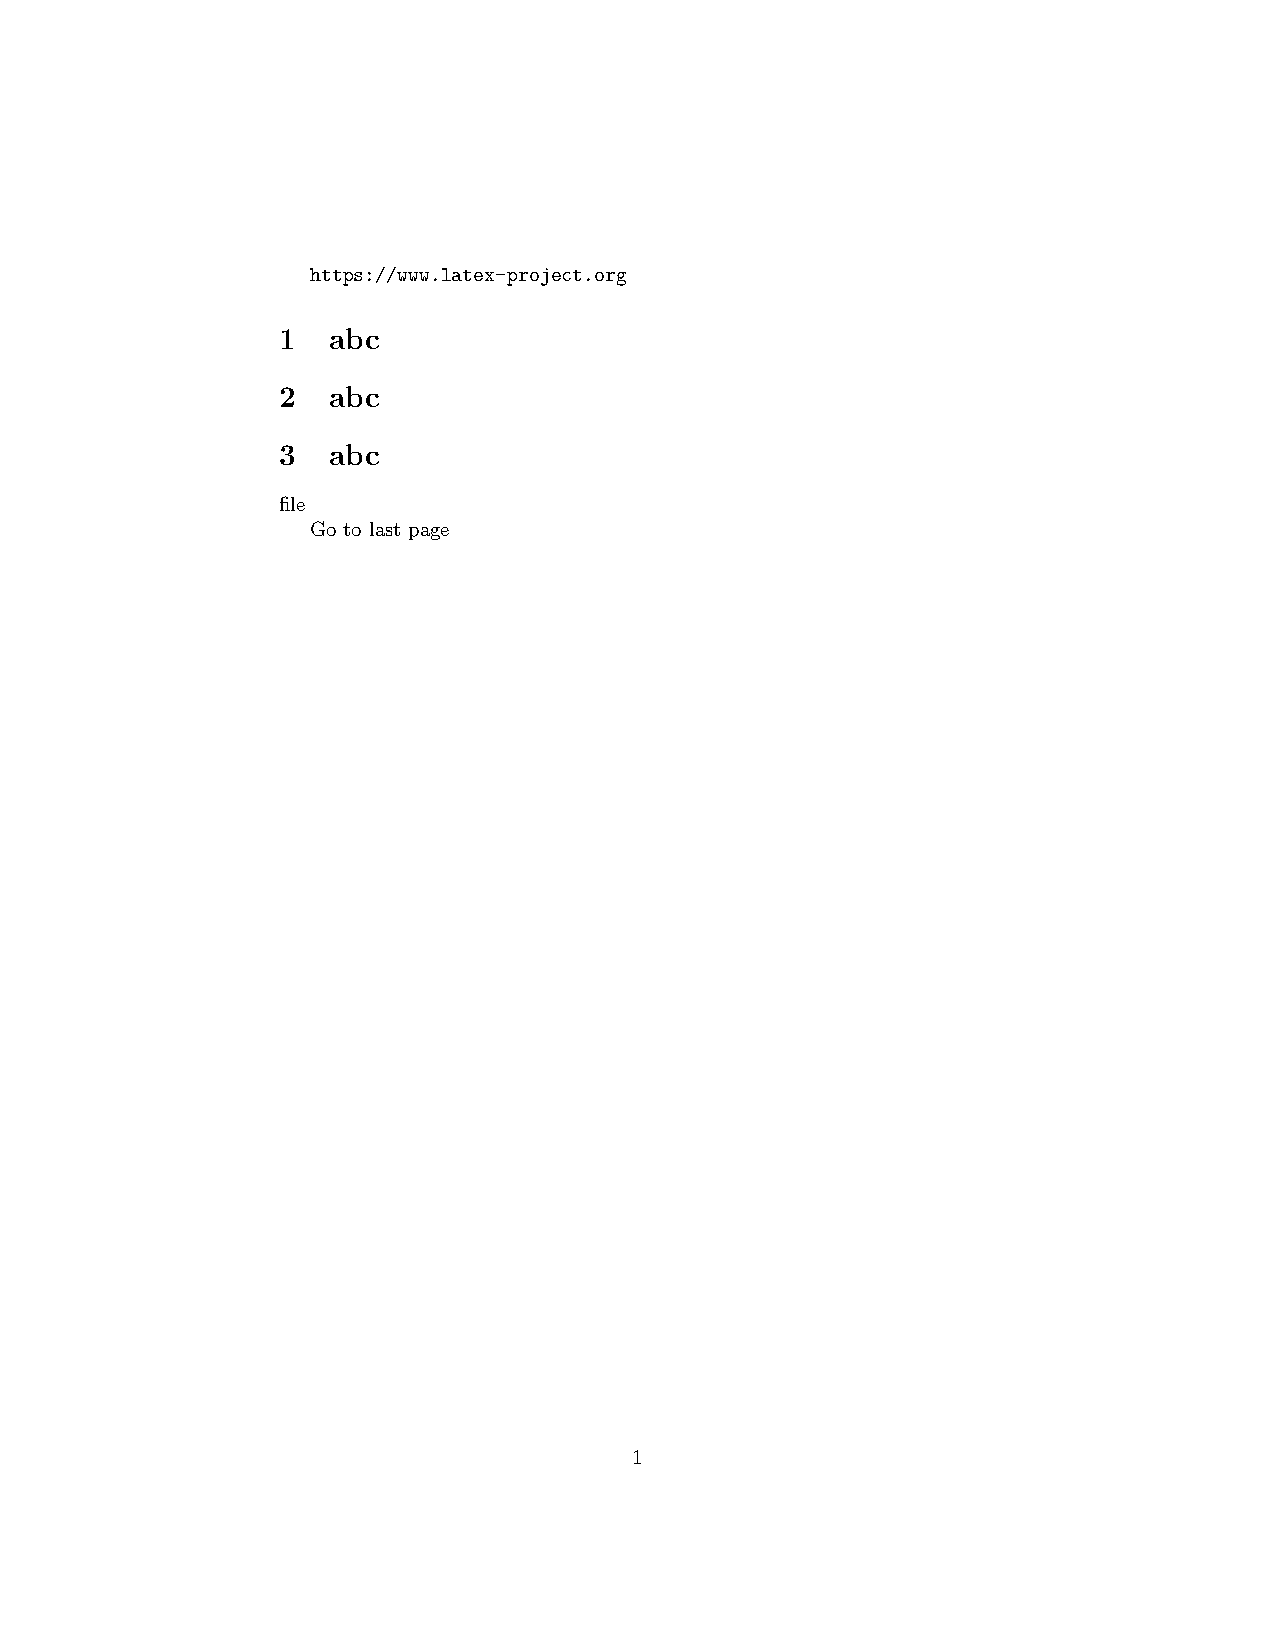
\includepdf[pages=-]{figure/pax-input2}
\end{document}
770 0 obj
<<
/Border [0 0 0]
/Subtype /Link
/Dest (G8.1935249)
/Type /Annot
/StructParent 716
/Rect [408.06 374.722 477 388.642]
>>
endobj
791 0 obj 